% \begin{figure}[h]
% \centering
% 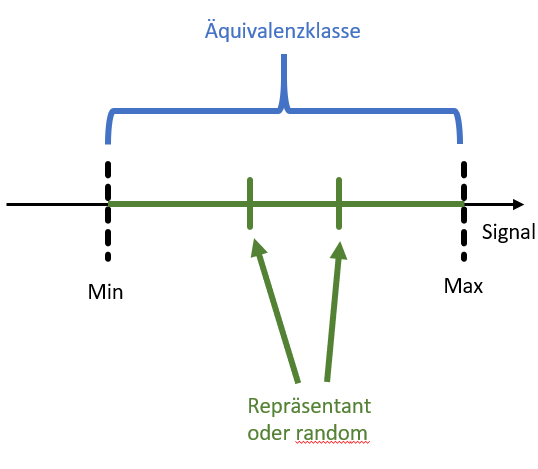
\includegraphics[scale=1.5,]{Bilder/EquiZeitstrahl/ZeitstrahlEineKlasse.png}
% \caption{Äquivalenzklasse in TPT}
% \end{figure}
%\textbf{Darstellung für random, Repräsentanten, Min und Max von Äquivalenzklassen in TPT}
Im \textit{Equivalence Class Set Editor} unter \textit{View} können Äquivalenzklassen definiert werden, um sie 
mehreren Signalen beziehungsweise einem einzigen Signal im Declaration Editor zuzuordnen.
%Die definierten Äquivalenzklassen können im zweiten Schritt Signalen zugeordnet werden.
Sie können als Assesslet \textit{Equivalence Classes} in der Auswertung der Testfälle eingesetzt werden.
%, um zu überprüfen, ob oder ob nicht bestimmte Klassen erreicht werden.
Sie können gleichermaßen in der Step Liste eingesetzt werden, um
Signale auf bestimmte Äquivalenzklassen zu setzen \parencite[S. 370 ff.]{userguide}.\\
\begin{description}
\item[Assessment]%Ein bild zum Assessment
Mit dem \textit{Equivalence Class Coverage table} können
ausgewählte Testfälle überprüft werden, ob Channels Werte ihrer Äquivalenzklassen
annehmen. In der Report Übersicht wird für jede Äquivalenzklasse der 
gewählten Channels angezeigt, ob und wie oft sie in den gewählten Testfällen vorkommen.
Eine weitere Möglichkeit im Assessment ist, dass 
man forbidden, also verbotene sowie mandatory, verpflichtende
Äquivalenzklassen festlegen kann. Eine Verbotene
besteht den Test, wenn sie nicht eintritt.
Eine Verpflichtende besteht den Test, wenn sie ein
oder mehrere Male eintritt \parencite[S. 1282 ff.]{userguide}.\\
% Eine verpflichtende Äquivalenzklasse
% kann für ausgewählte 
% Testfälle Channels gesetzt werden. Diese Channels, die Äquivalenzklassen besitzen,
% werden darauf überprüft, ob sie  
% Es wird ein Signal ausgewählt, man kann zwischen mandatory, forbidden und .. auswählen.
% Oben sind 4 Haken zu setzen, diese hier erklären.
\item[Step Liste]%\%ein Bild zur Step Liste
Es gibt vier Schlüsselwörter, um eine Äquivalenzklasse eines Channels
in der Step Liste zu benutzen: \textit{Random, representative, min} und \textit{max}.
Mit \textit{min} und \textit{max} sind jeweils die Grenzen des definierten Wertebereichs gemeint. Mit \textit{random} wird ein zufälliger Wert gewählt, mit \textit{representative} ein Repräsentant.
Wenn kein Schlüsselwort angegeben wird, so wird der Repräsentant gewählt.
Falls kein Repräsentant definiert ist, so wird ein zufälliger Wert innerhalb des Wertebereichs
gewählt \parencite[S. 379 f.]{userguide}.\\
\item[Äquivalenzklassen von TPT generieren lassen]
Dies kann man mit \textit{Generate Test Cases -> from Equivalence Classes} erreichen.
Man kann auswählen ob sie in einer Step Liste nacheinander
geschrieben werden oder jede in einer 
eigenen Step Liste. Weitere Einstellungsmöglichkeiten sind eine paarweise Kombination und Grenzwerte (siehe Abschnitt 2.2) \parencite[S. 668 ff.]{userguide}. 
\end{description}
% Generate Test Cases -> from Equivalence Classes 
% Optionen: Auswählen ob Äquivalenzklassen in einzelnen Testfällen, oder alles in einen Testfall als Sequence geschrieben werden

% % Wie erstellt man Äquivalenzklassen in TPT?
% % View -> Equivalence Class Set Editor, Signal in Wertebereich einteilen
% % View -> Declaration Editor Channel(Signal) auf definierte Äquivalenzklasse setzen
% % Assessment -> Equivalence Class auswählen
% % Signale auswählen, mandatory und forbidden equi classes eingeben

% % fertig, jetzt Testdurchführung

% % Äquivalenzklassen von TPT generieren lassen:
% % Generate Test Cases -> from Equivalence Classes 
% % Optionen: Auswählen ob Äquivalenzklassen in einzelnen Testfällen, oder alles in einen Testfall als Sequence geschrieben werden

% % Möglichkeiten der Test Case Erstellung mit Äquivalenzklassen
% % mit Signal.ec->high etc., Repräsentanten und andere Funktionen

% % Dieses Kapitel zu TPT Analyse